\chapter{Static networks, homogeneous mean field approximation}

\resp{Veronica Bedin}

\section{Epidemics modeling}
Epidemic modeling began with Kermack and McKendrick’s 1927 work \cite{kermack1927contribution} and became a key tool in epidemiology. Its role was pivotal during COVID-19 for tracking transmission and guiding interventions \cite{ferguson2020impact, flaxman2020estimating, giordano2020modelling}. Compartmental models are the most widely used approach, aiming to describe population-level dynamics from individual contagion processes. Each individual is in state $n$ at time $t$. \\
Depending on the model we are considering, the states are different:
\begin{enumerate}
    \item \textbf{S}: susceptible, the individual is healthy but susceptible to the disease
    \item \textbf{E}: exposed, the individual has been exposed to the disease.
    \item \textbf{I}: infected, the individual is ill and capable of infection. 
    \item \textbf{R}: recovered, the individual recovered from the illness (or died) and is no longer infectable. 
\end{enumerate}
 
The most widely used compartmental models are the following:
\begin{enumerate}
    \item \textbf{\textit{SI}}:
        The \textit{SI} model is applicable to diseases in which recovery does not occur. The population is divided into susceptible $S$ and infected $I$. The infection process is modeled by the reaction: $$S+I\xrightarrow{\beta}I+I$$ $\beta$  is the probability per unit of time that an individual S becomes I upon contact with an individual I. 
    \item \textbf{\textit{SIS}}:
        The \textit{SIS} model applies to infections that do not confer lasting immunity. In this case, individuals return to the susceptible compartment after recovery: $$S+I\xrightarrow{\beta}I+I$$ $$I\xrightarrow{\mu_S}S$$
        $\mu_S$, is the rate at which an individual becomes S again, the inverse of infection time $\tau_I$.
    \item \textbf{\textit{SIR}}:
        The \textit{SIR} model applies to infections that confer lasting immunity (or death). In this case, individuals move to the recovered compartment after recovery: $$S+I\xrightarrow{\beta}I+I$$ $$I\xrightarrow{\mu_R}R$$
        $\mu_R$, the rate at which an individual recovers, the inverse of infection time $\tau_I$, where $\tau_I$ is the duration of infection.  
    \item \textbf{\textit{SEIR}}:
        The \textit{SEIR} model incorporates a latent period between exposure and infectiousness: individuals do not become infectious immediately after being infected.

        $$S+I\xrightarrow{\beta}I+E$$
        $$E\xrightarrow{\alpha}I$$
        $$I\xrightarrow{\mu}R$$
        $\beta_E$ is the \textit{exposion rate}. $\alpha$ is the rate at which an individual becomes infected, the inverse of exposion time $\tau_E$. 
\end{enumerate}

Some quantities of interest in epidemic modeling include:
\begin{itemize}
\item The \textit{basic reproduction number} $R_0$ average number of secondary infections produced by a single infected individual in a fully susceptible population.
\item \textit{Effective reproduction number} $R(t)$: secondary cases per case at time $t$.
\item \textit{Critical epidemic threshold}: the critical value of parameter $\beta$ above which an epidemic can invade the network.
\end{itemize}

\section{Homogeneous Mean-Field Approximation}

The objective of this review is to simulate the behavior of well-known epidemic models and analyze their dynamics, particularly focusing on critical phenomena such as the epidemic threshold. To do so, I compare computational simulations run on networks with analytical predictions derived under the \textit{homogeneous mean-field} (HMF) approximation. This approximation assumes a network with bounded or uniform degree, i.e., $k_i \simeq \langle k \rangle$, allowing each node to be treated statistically equivalently.

A deeper treatment of the models and governing ODEs is provided in Appendix~\ref{app:Homogeneous_MF}, where \textit{SI}, \textit{SIR}, and \textit{SEIR} are described. Here, I focus on the \textit{SIS} model, both analytically and via simulation.

\subsection{\textit{SIS} Dynamics on Homogeneous Networks}
To formulate the \textit{SIS} model on a general network, we define a binary state variable $\sigma_i(t)$, which is $1$ if node $i$ is infected and $0$ if susceptible. Let $\rho(i,t) = \text{Prob}[\sigma_i(t) = 1]$. The evolution equation is:
\begin{equation}
\frac{d\rho(i,t)}{dt} = -\mu \rho(i,t) + \beta \sum_j A_{ij} \text{Prob}[\sigma_i(t)=0,\sigma_j(t)=1]
\label{eq:SIS_network_dynamics}
\end{equation}

This form is not closed due to correlations between neighbors. Under the HMF approximation and assuming spatial homogeneity $\rho(i,t) = \rho(t)$, we factor the joint probability: $\text{Prob}[\sigma_i=0,\sigma_j=1] \approx (1-\rho)\rho$. Equation~\eqref{eq:SIS_network_dynamics} becomes:
\begin{equation}
\frac{d\rho}{dt} = -\mu\rho + \beta \langle k \rangle (1 - \rho) \rho
\label{eq:SIS_network_dynamics_hom}
\end{equation}
Throughout this work, in all specific model analyses, we set $\mu_S = \mu$ or $\mu_R = \mu$ to simplify the notation without loss of generality.

For a detailed derivation of these calculations, see Appendix~\ref{app:full_counts}.

This mean-field ODE predicts an epidemic threshold at $\beta_c = \mu / \langle k \rangle$. For $\beta > \beta_c$, an endemic equilibrium $\rho^* > 0$ is reached.

\subsection{Comparison with Simulations}
I simulate the \textit{SIS} model on an Erd\H{o}s-Rényi network with $N=10000$ and average degree $\langle k \rangle \approx 8$. The simulation implements the stochastic infection and recovery process node by node. 
Further information about the simulation process can be found in Section \ref{app:Numerical_simulations}. Snapshots and density evolution are shown below.

\begin{figure}[H]
\centering
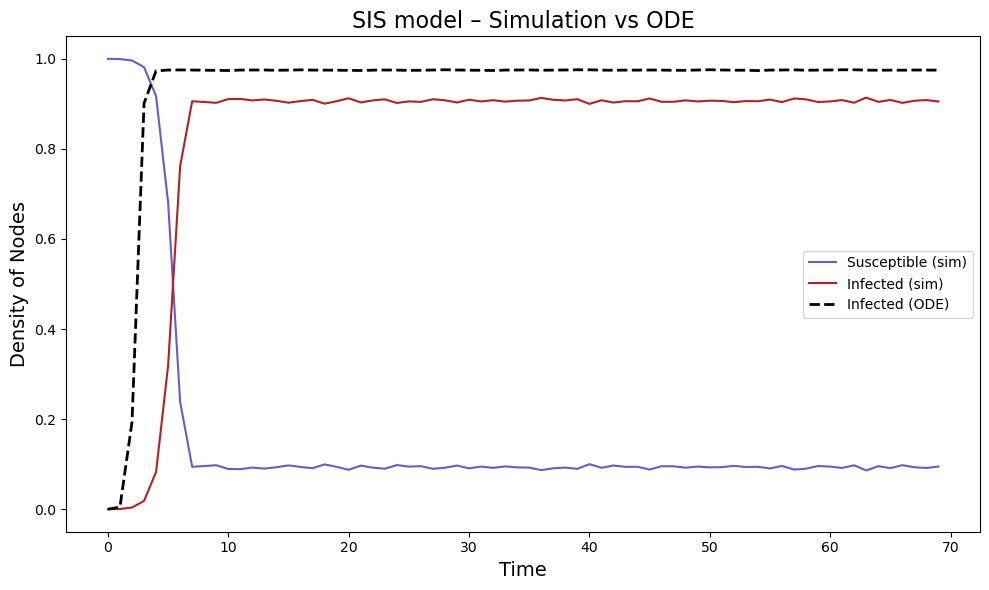
\includegraphics[width=0.6\textwidth]{images/Homogeneous/SIS_densities.png}
\caption{Time evolution of the density of susceptible (blue) and infected (red) individuals. In black the analytical Homogeneous MF evolution of the infected.}
\label{fig:SIS_densities}
\end{figure}

The simulation results exhibit a non-zero steady-state infected density, qualitatively consistent with the ODE prediction in Equation~\eqref{eq:SIS_analytical_full}. However, noticeable differences between the analytical and simulated curves appear even at early times. These deviations are primarily due to finite-size effects and stochastic fluctuations which are not captured by the mean-field approximation.

Here, I focused on the \textit{SIS} model. The remaining models (\textit{SI}, \textit{SIR}, \textit{SEIR}), along with their governing equations and analytical solutions, are provided in Section~\ref{app:Homogeneous_MF}.

\subsection{Threshold Estimation}
I also numerically estimate the critical threshold $\beta_c$ by running the simulation for increasing $\beta$ ($10$ times for each $\beta$) and observing whether the infection dies out or reaches an endemic state. 
Figure~\ref{fig:threshold} illustrates the epidemic threshold for the \textit{SIS} model by comparing the simulated infected density with the analytical prediction. The theoretical threshold is \(\beta_c = 0.005\), very close to the one obtained in the simulations.

I do not include similar threshold plots for the other models: in the \textit{SI} model, the concept of a threshold is not meaningful because infection spreads irreversibly without recovery, while the \textit{SIR} and \textit{SEIR} models display a threshold behavior qualitatively similar to the \textit{SIS} case.


\begin{figure}[H]
\centering
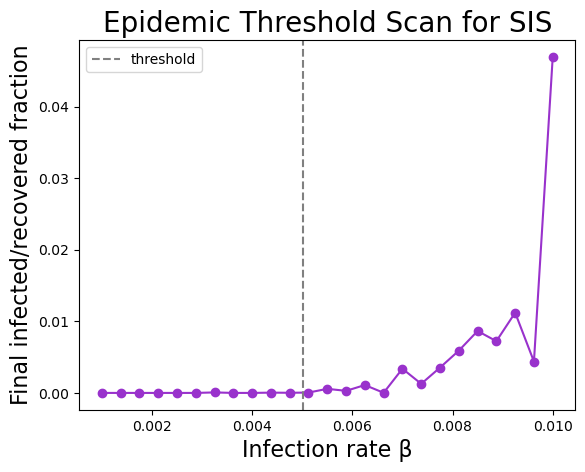
\includegraphics[width=0.6\textwidth]{images/Homogeneous/SIS_threshold.png}
\caption{Steady-state of infected density as a function of $\beta$. The gray line is the theoretical threshold}
\label{fig:threshold}
\end{figure}

In simulations, the observed threshold is compatible with the one we obtain through theory. At $\beta_c = 0.005$ we observe the first onset of the disease.





\newpage